\section{Part 2: Cardiac Signal (ECG)}

\begin{taskbox}[Part 2: introduction in the lab manual]
A segment of ECG recorded from two leads is provided in the file \texttt{sig\_ECG.mat}. This signal is record number 201 of the MIT-BIH Arrhythmia database. More details about this database can be found in the file \texttt{Introduction\_Arrhythmia.pdf}. The signals recorded in this database belong to healthy and diseased subjects over a duration of 30 minutes, and the R-peak location and the label of each beat (normal/abnormal and its type) are specified.
\end{taskbox}

\subsection{Question 1: Displaying Two Leads and Comparing Beat Shapes}
\begin{taskbox}
Plot the signals of the two channels in time (stored in the matrix \texttt{Sig} with sampling frequency \texttt{sfreq}). The time axis must be displayed in seconds. By zooming on the horizontal axis, examine the changes of the signals of the two channels over time. Are the beats similar to each other over time in each channel? Are the beats of the two channels similar? Plot two sample (different) beats and mark the P, Q, R, S and T waves on them.
\end{taskbox}

The cardiac data belong to record 201 of the MIT-BIH Arrhythmia database. According to the original header, the two leads are MLII and V1, and the sampling rate is 360~Hz. The stored amplitude is consistent with a calibration of 200~ADU/mV and a baseline of 1024; for example, the initial digital values 972 and 982 convert to $-0.26$~mV and $-0.21$~mV, which match the first row of the data. The amplitude axis of this part is therefore in millivolts.

\begin{figure}[H]
\centering
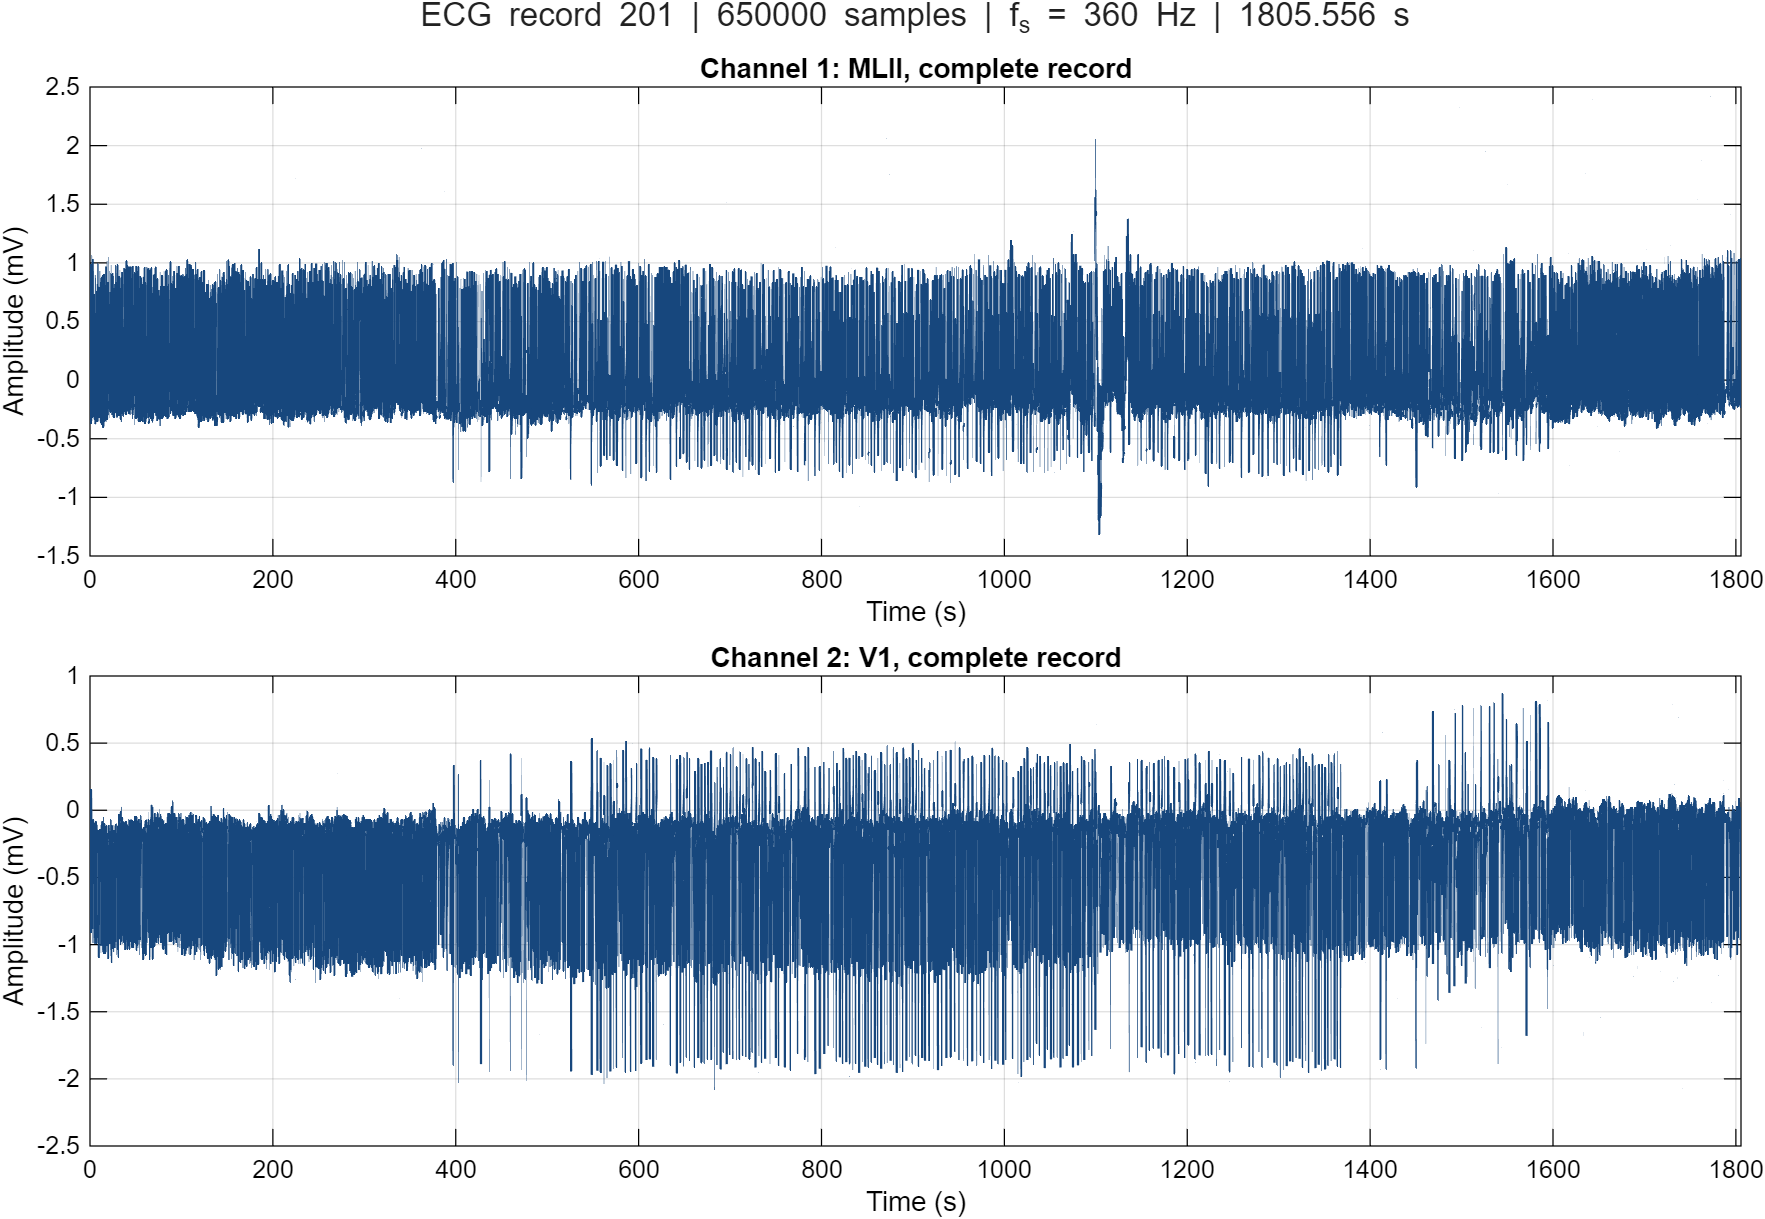
\includegraphics[width=0.95\textwidth]{fig12_ecg_full_record.png}
\caption{Complete recording of the two cardiac leads, with the time axis reconstructed from the real length of the signal.}
\label{fig:ecgfull}
\end{figure}

Figure~\ref{fig:ecgfull} gives the overall view of the recording, and Figure~\ref{fig:ecgseg} shows enlarged segments. The time of occurrence of the cardiac complexes is common to the two leads, because both record the same heart; the shape, amplitude and polarity, however, are not the same. In MLII a positive R wave is usually prominent, whereas in V1 a small r and a larger negative S component are seen. The change of the viewing axis and the location of the electrodes explain this difference.

The beats of a single lead are also not completely similar over the whole recording. At the start of the recording the intervals are irregular, at about 397.6 seconds there is a ventricular sample with a different shape, and at about 1430 seconds several beats with N shape are seen more regularly. The N label specifies the usual shape of the complex; by itself it does not mean sinus rhythm or the health of the whole recording. According to the original description of the data, the recording begins with atrial fibrillation.

\begin{figure}[H]
\centering
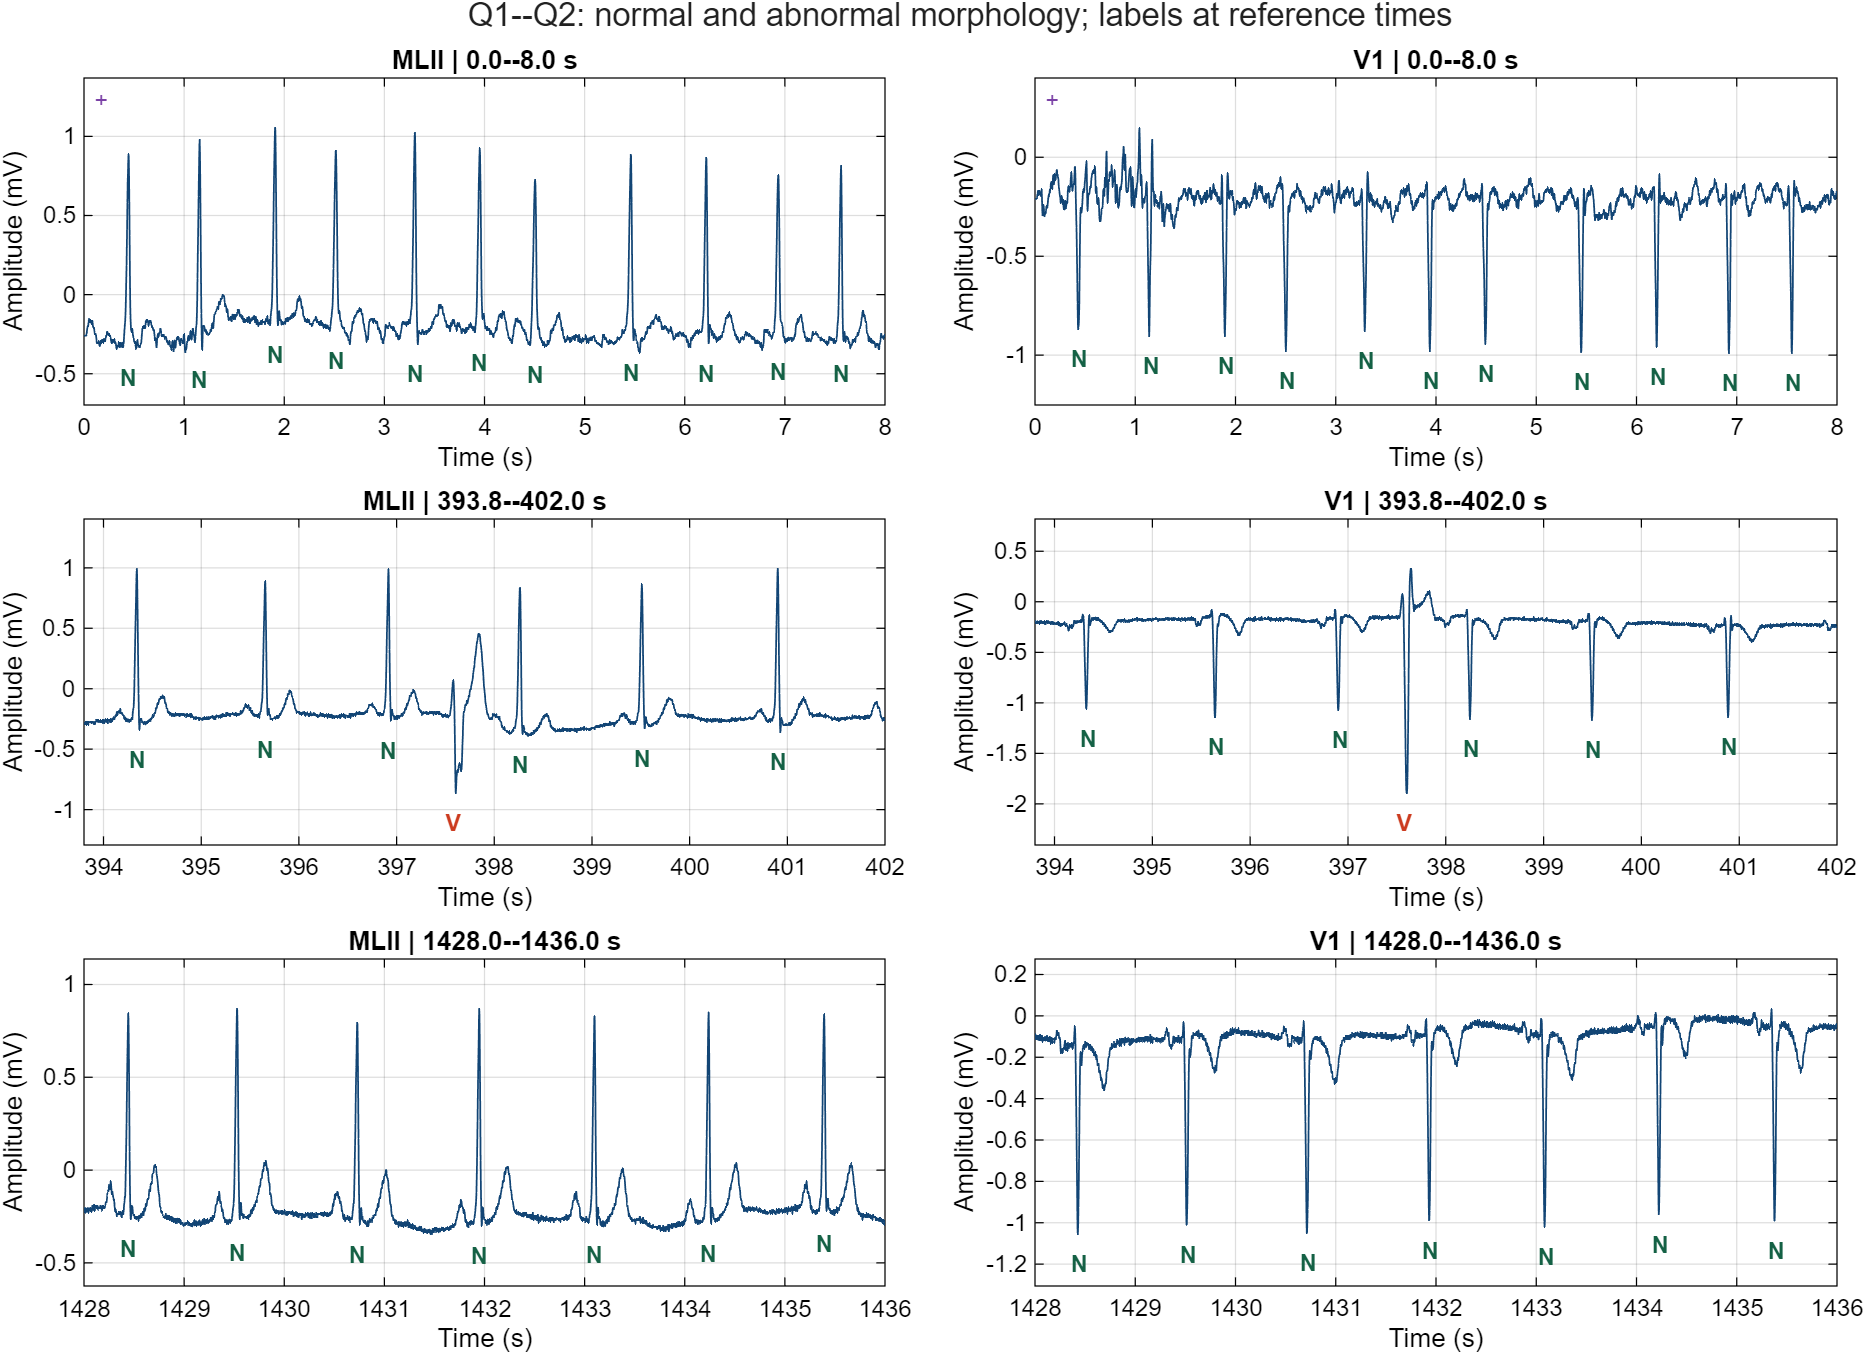
\includegraphics[width=\textwidth]{fig13_ecg_segments_with_labels.png}
\caption{Readable segments of the two leads at three different times, with the reference beat labels shown.}
\label{fig:ecgseg}
\end{figure}

For two different beats, an N sample at 1430.725~s and a V sample at 397.578~s were chosen. In Figure~\ref{fig:pqrst}, the distinguishable waves are marked for instructional purposes. The small q/s peaks are not definite in some leads; the absence of a distinguishable component must not be filled in with an artificial marker. In the ventricular sample, an independent P wave is not clear and Q has not been determined separately. The time markers are not valid clinical boundaries for measuring PR or QT.

\begin{figure}[H]
\centering
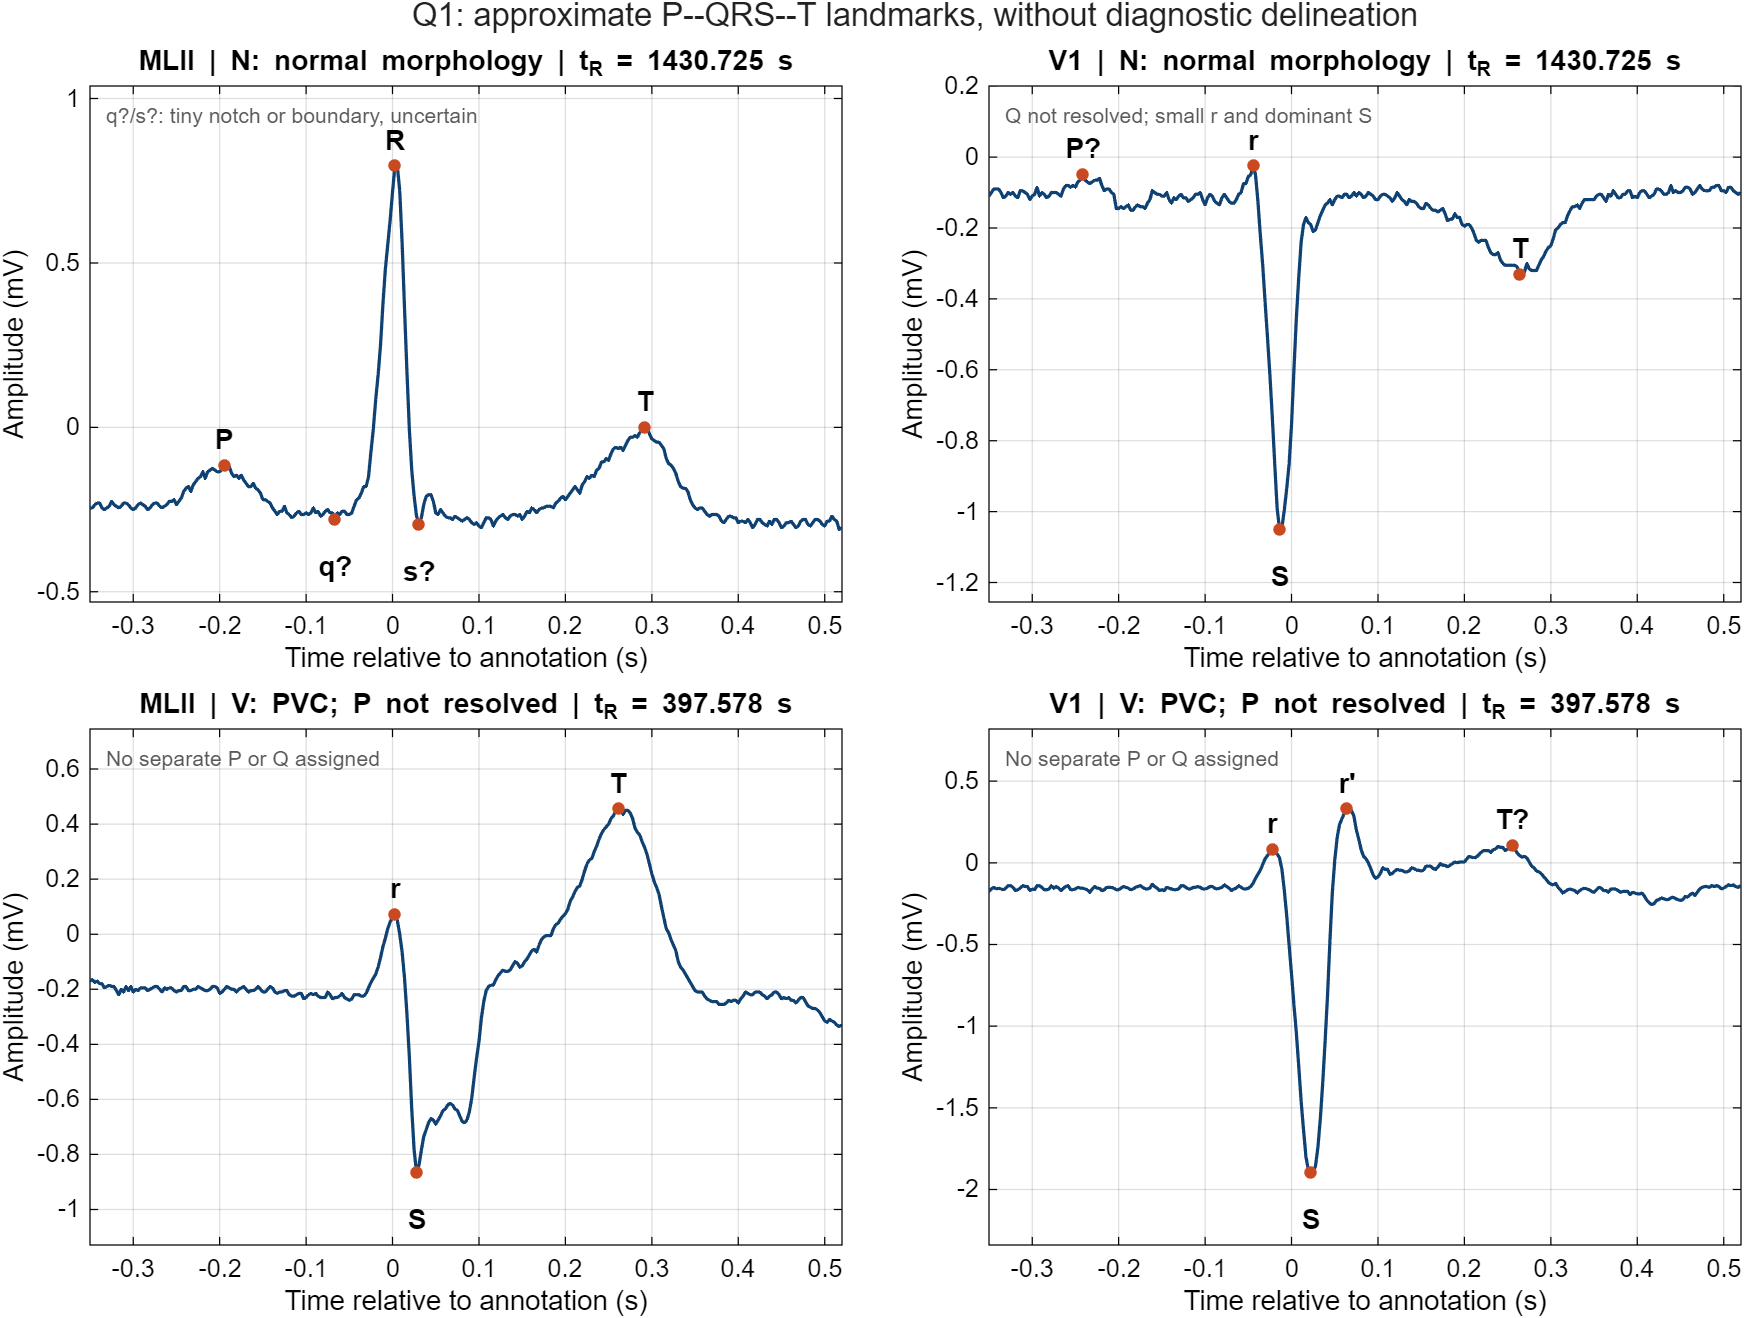
\includegraphics[width=\textwidth]{fig14_ecg_pqrst_landmarks.png}
\caption{Approximate marking of the distinguishable waves in two different beats and two leads.}
\label{fig:pqrst}
\end{figure}

The P wave is atrial activity, the QRS complex is ventricular depolarization, and the T wave is ventricular repolarization. Not all beats necessarily show all five letters as separate, clear peaks or troughs. In addition, the reference time of the database label is the characteristic time of the complex; in the second lead it may not lie exactly on the positive peak of R.

\subsection{Question 2: Interpreting Labels and Labeling All Beats}
\begin{taskbox}
The occurrence time of the R wave is given in the vector \texttt{ATRTIMED} and the type (abnormality) of the beat in the vector \texttt{ANNOTD}. The number 1 in \texttt{ANNOTD} indicates a normal beat, and every other number indicates a type of abnormality. The abnormality corresponding to each number is described in the file \texttt{ANNOTATIONS.pdf}. For the signal of each channel, write the abnormality type of each beat below it (at the time of the R peak). You can use the \texttt{text} command.
\end{taskbox}

The vectors \texttt{ATRTIMED} and \texttt{ANNOTD} give the event time and the event code, respectively. To convert time to a MATLAB index, \texttt{round(t*fs)+1} was used. The exact definition of the codes was taken from the accompanying file \texttt{ANNOTATIONS.pdf} and from the official WFDB reference. Contrary to the simplification in the exercise statement, a number other than one is not always an abnormal beat: codes 14, 28 and 37 mark a signal quality change, a rhythm change and a non-conducted atrial wave, respectively.

\begin{center}
\begin{tabularx}{\textwidth}{@{}cc>{\raggedright\arraybackslash}Xcc@{}}
\toprule
\textbf{Code} & \textbf{Symbol} & \textbf{Meaning of the event} & \textbf{Count} & \textbf{Ventricular complex}\\
\midrule
1  & N & Beat with the usual shape & 1625 & Yes\\
4  & a & Aberrated atrial premature beat & 97 & Yes\\
5  & V & Premature ventricular beat & 198 & Yes\\
6  & F & Fusion of ventricular and normal beat & 2 & Yes\\
7  & J & Premature junctional beat & 1 & Yes\\
8  & A & Premature atrial beat & 30 & Yes\\
11 & j & Junctional escape beat & 10 & Yes\\
14 & $\sim$ & Signal quality change & 4 & No\\
28 & + & Rhythm change & 35 & No\\
37 & x & Non-conducted premature atrial wave & 37 & No\\
\bottomrule
\end{tabularx}
\end{center}

In total there are 2039 events, but the number of actual ventricular complexes is 1963: 1625 N beats and 338 beats with a non-N shape, i.e.\ about 17.22\% of the beats. The 76 remaining events were not included in the computation of the RR intervals. The mean RR interval is about 0.920~s, the median is 0.863~s, and the range is 0.336 to 3.772~s. The heart rate over the whole duration of the recording is about 65.23 beats per minute; this ratio is not the same quantity as the arithmetic-mean-based $60/\mathrm{RR}$.

All 1963 beats were labeled with their reference times in both leads in the appendix file \texttt{figures/ecg\_all\_beats\_annotated.pdf}. The appendix has 61 pages, and each page shows three ten-second cuts of both leads, so that all labels are legible. The beat symbol is placed under the complex, and a non-beat event is placed above the signal. Figure~\ref{fig:ecgseg} shows examples of the labeling in the body of the report.

\subsection{Question 3: Comparing All Beat Types and Explaining Their Mechanisms}
\begin{taskbox}
Extract one or more beats of the normal type and of each abnormality, and compare their temporal-morphological features. By searching the internet, briefly explain how each type of abnormality present in this recording arises and what its characteristics are.
\end{taskbox}

For each beat type, several aligned examples and the median pattern were plotted. To compare shapes, the baseline of each segment was shifted, but the original signal was not filtered or rewritten. To prevent a neighboring beat from entering the segment, its extent was limited to half the distance to the neighbors. Figures~\ref{fig:beats1} and~\ref{fig:beats2} show the differences between the waveforms. For J only one sample, and for F two samples, exist; from such small numbers we do not infer a stable statistical result for a population.

\begin{figure}[H]
\centering
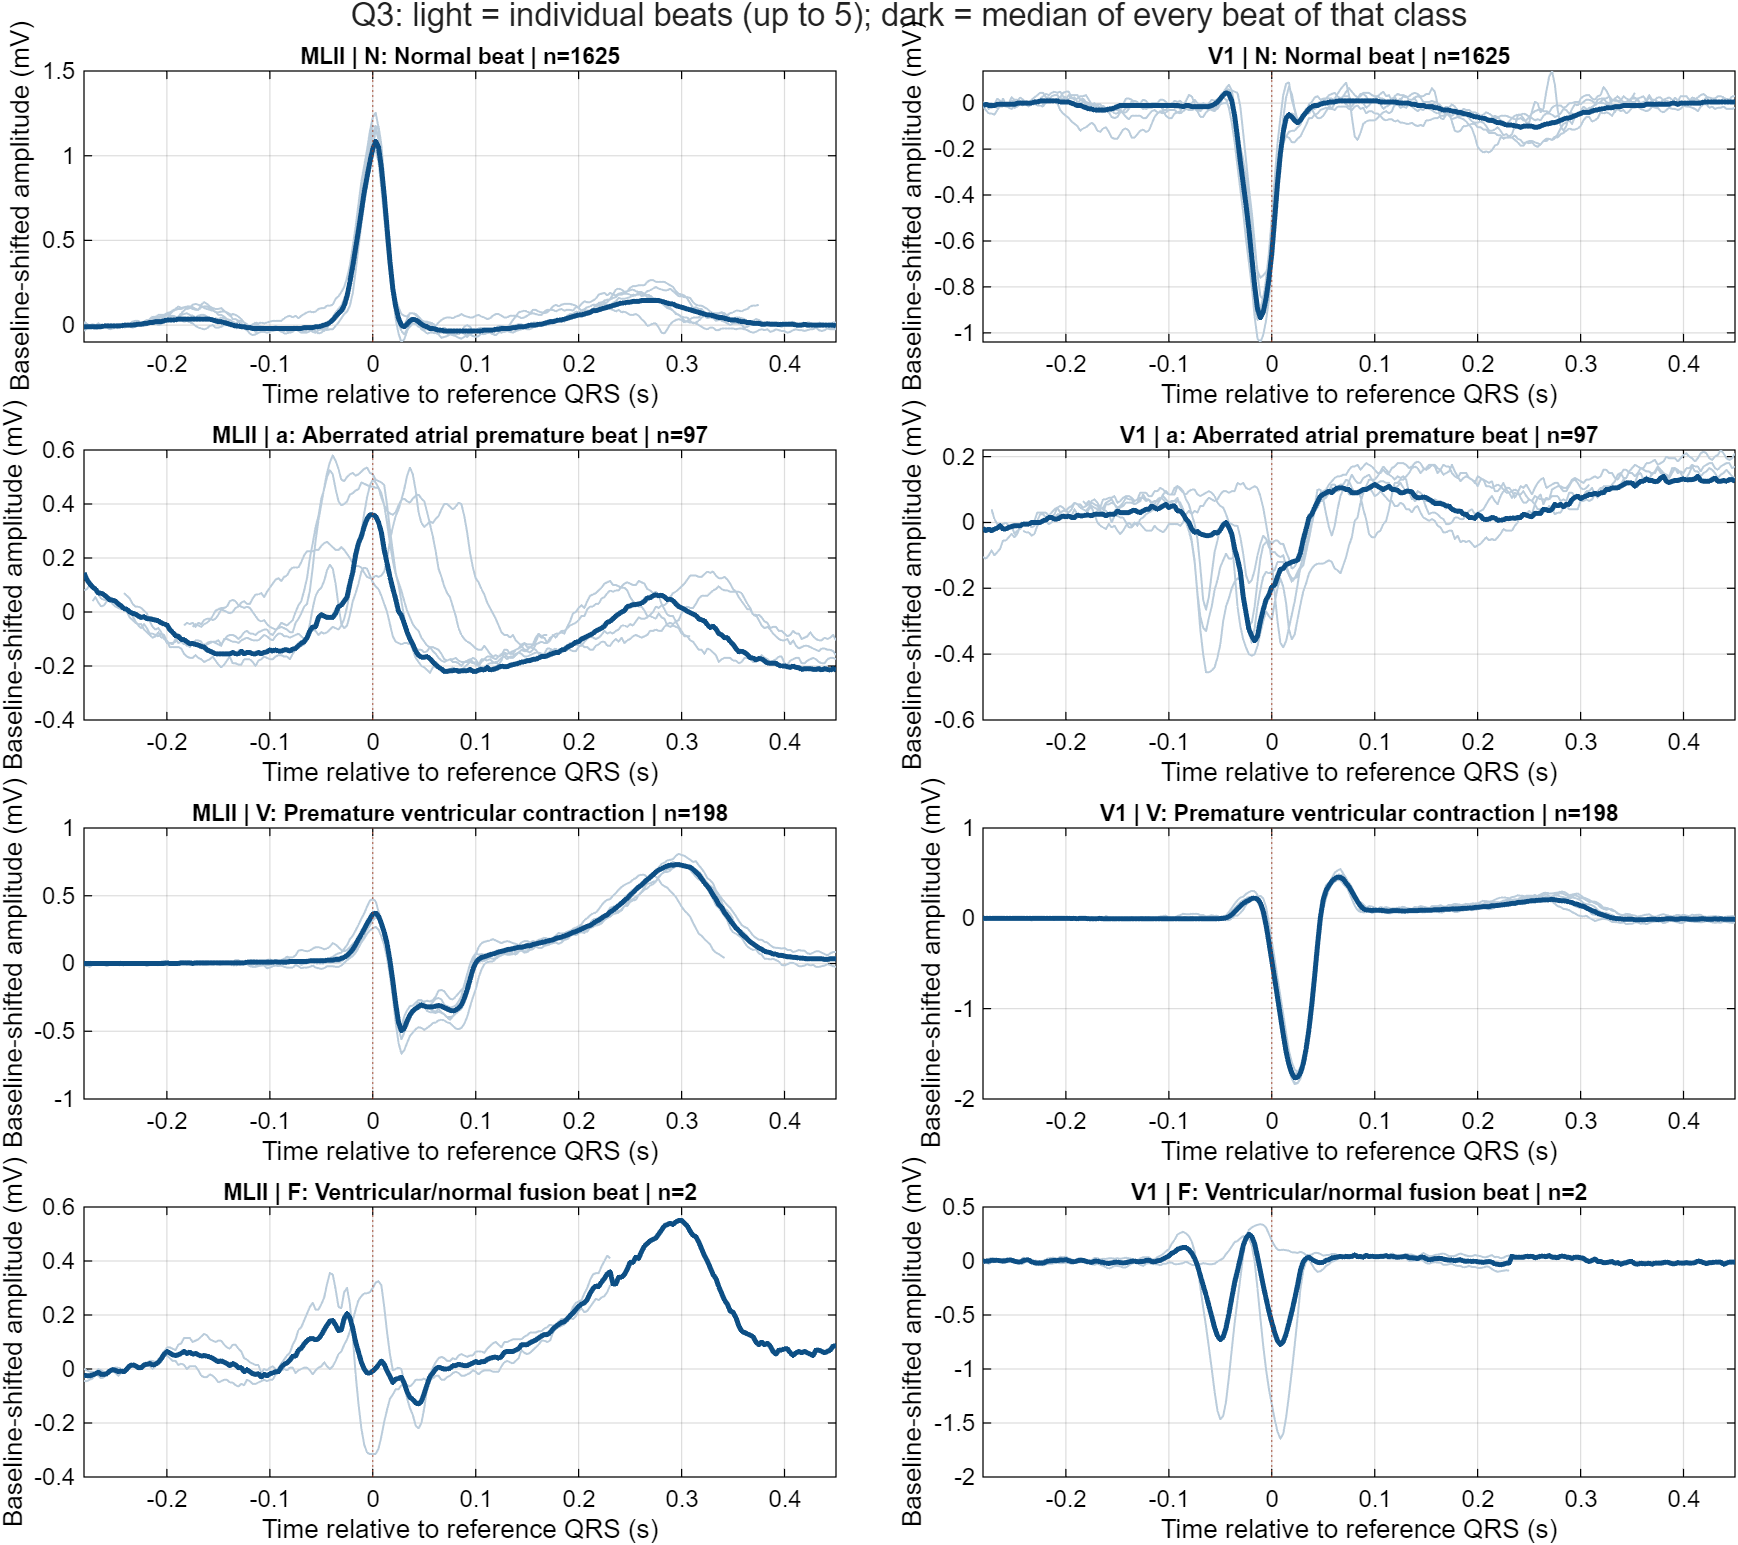
\includegraphics[width=0.95\textwidth]{fig15_beat_classes_n_a_v_f.png}
\caption{Examples and median shape of the normal beat and of the aberrant atrial, ventricular and fusion beats.}
\label{fig:beats1}
\end{figure}

\paragraph{Premature atrial beat and aberrant conduction (A and a).} In A, the stimulus starts from an atrial focus earlier than the expected beat. If ventricular conduction remains usual, the QRS can be close to that of N, and the difference is seen more in the timing and in the atrial wave. In a, the same premature atrial stimulus appears with a shape-changed QRS because of the conduction state of the bundle branches; widening of the complex alone is therefore not sufficient to call it a ventricular beat. A premature atrial stimulus may be accompanied by usual conduction, aberrant conduction or complete conduction block.

\paragraph{Premature ventricular beat (V).} In V, the ventricular stimulus does not start from the usual upstream path, and its different propagation can create a wider complex and a different return of polarity. In our data, the median shape in MLII differs from N, and the negative component and the wave after it are more prominent; the median peak-to-peak amplitude in V1 is about 2.22~mV, compared with 0.98~mV for N. Possible mechanisms of ectopic ventricular excitation include automaticity, triggered activity and re-entry; the two leads of this experiment do not determine the cellular mechanism of each event.

\paragraph{Fusion beat (F).} In F, the usual and the ectopic ventricular activation take part simultaneously in forming the complex, and the final shape can have intermediate features.

\begin{figure}[H]
\centering
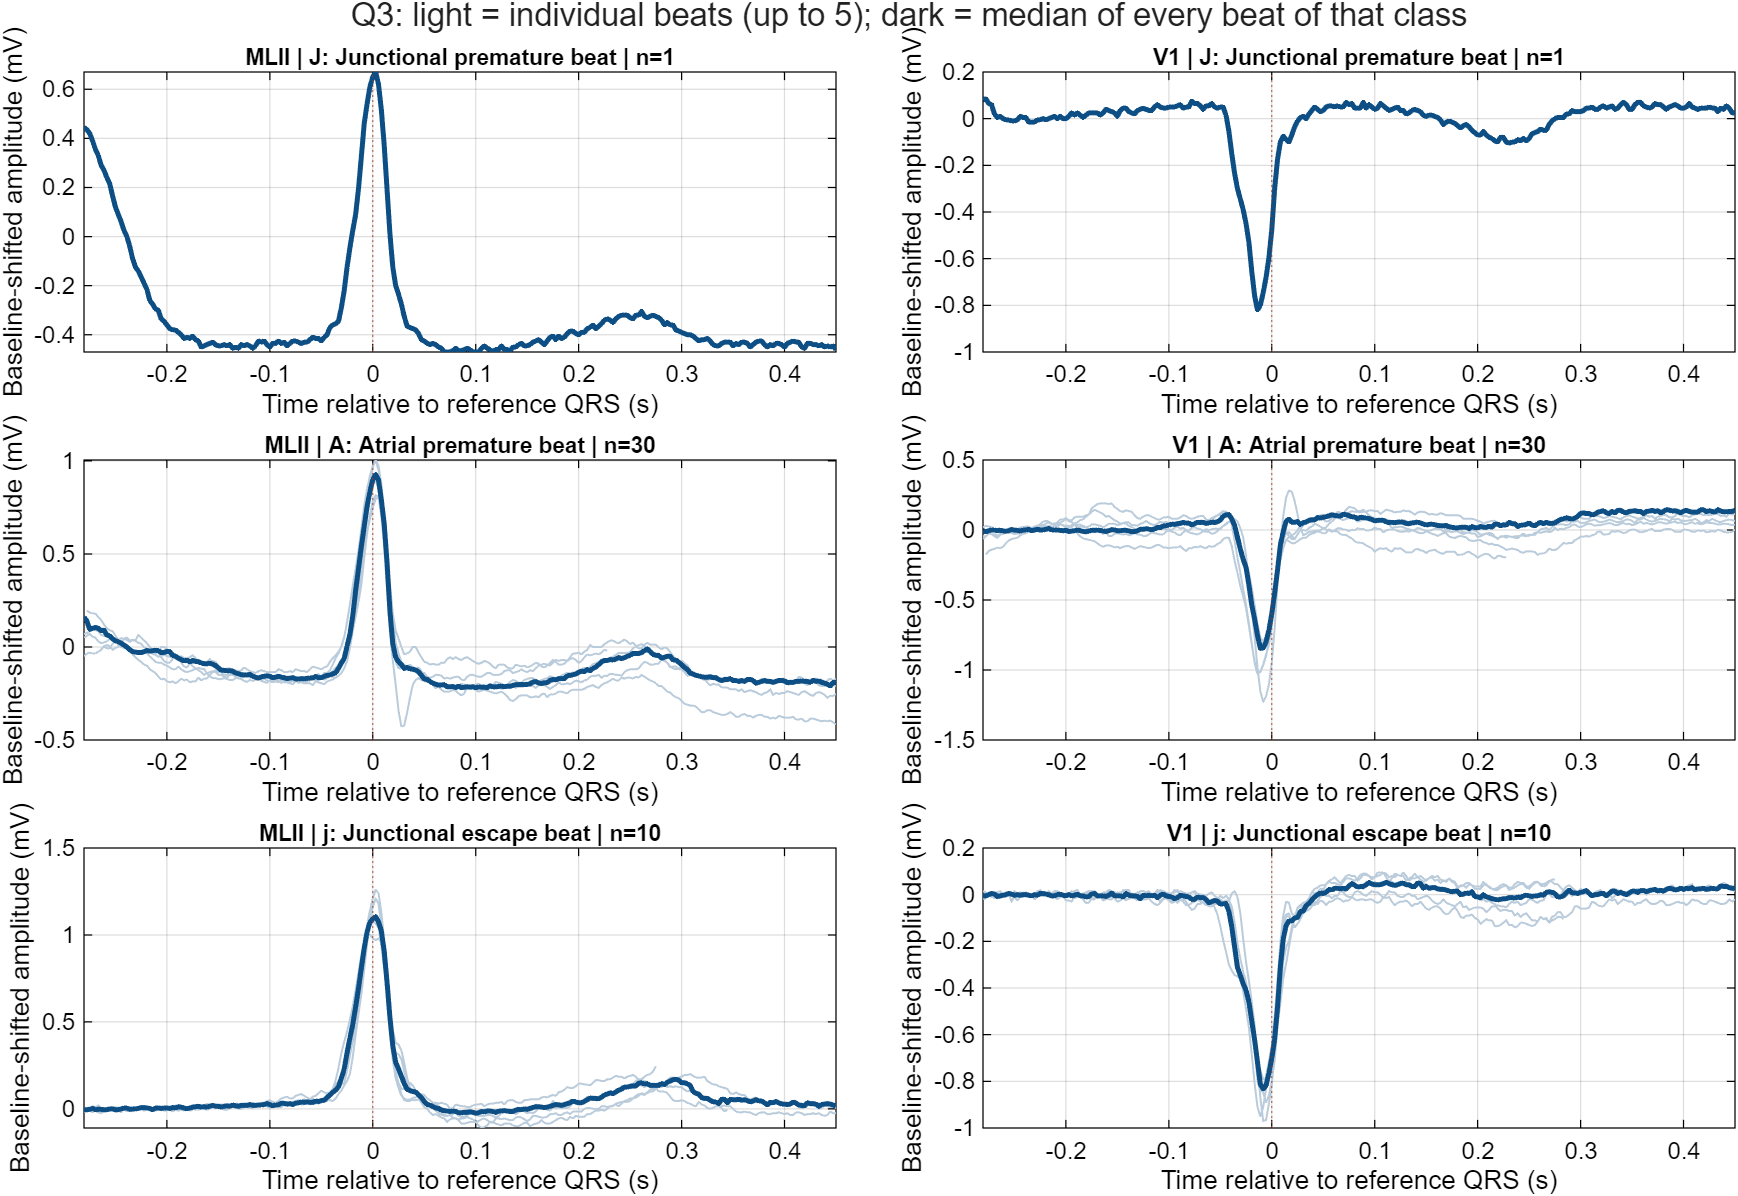
\includegraphics[width=0.95\textwidth]{fig16_beat_classes_j_A_j.png}
\caption{Examples and median shape of the junctional and atrial beats in the two leads.}
\label{fig:beats2}
\end{figure}

\paragraph{Junctional beats (J and j).} In J, the stimulus is a premature junctional one, whereas j is an escape beat after a delay in the upstream activation. Depending on the path and the conduction time, the QRS may be close to that of N, and the atrial wave may be absent, hidden or of different polarity. In the present data, the median preceding interval of J is about 0.575~s and that of j about 1.901~s; this difference is consistent with the distinction between premature and escape beats.

\paragraph{Non-conducted atrial wave (x).} The marker x belongs to a premature P wave that did not produce the next ventricular complex; for example, the stimulus can arrive while the conduction path is refractory. Figure~\ref{fig:blocked} shows an example in the context of the two leads. This event is physiologically important, but counting it as an R wave creates a false short interval in the computation of the heart rate.

\begin{figure}[H]
\centering
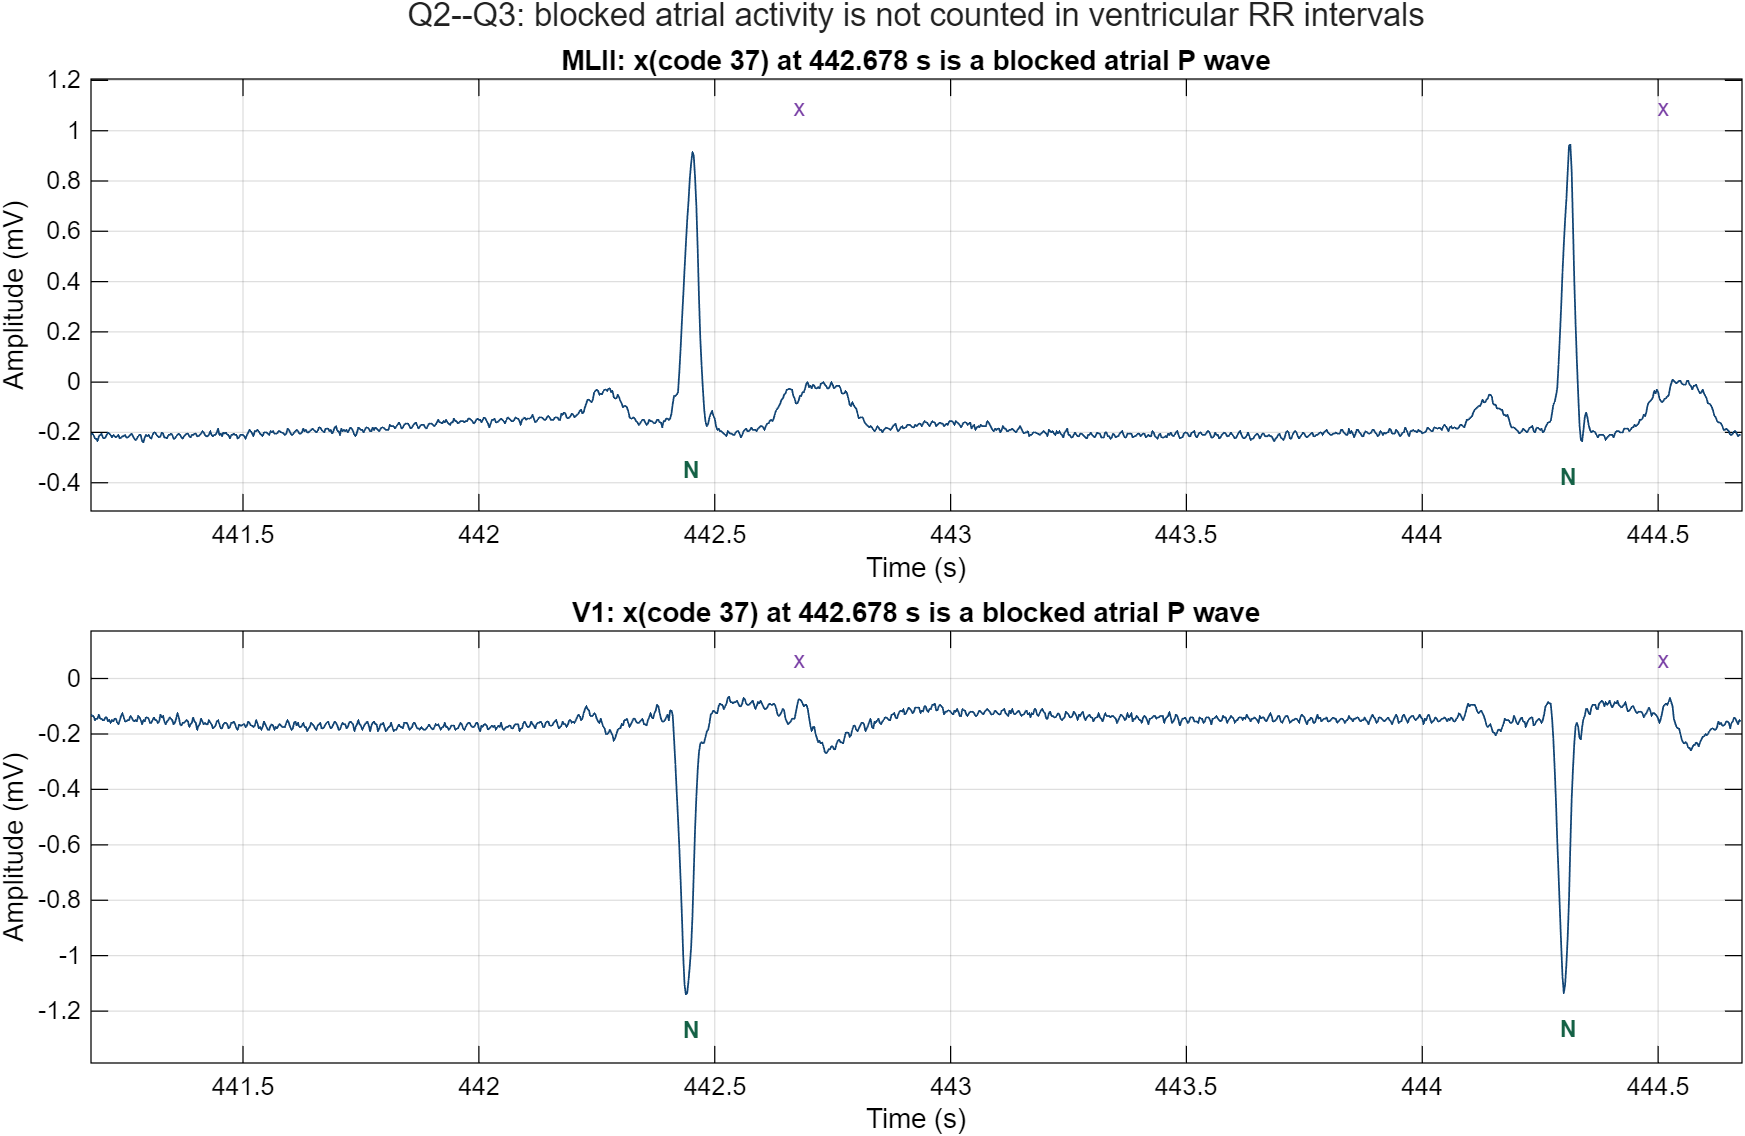
\includegraphics[width=0.95\textwidth]{fig17_blocked_atrial_wave.png}
\caption{A sample of a non-conducted atrial wave in the context of the two leads, and its separation from the ventricular beat.}
\label{fig:blocked}
\end{figure}

\subsection{Question 4: Comparing Two Segments of Three Consecutive Beats}
\begin{taskbox}
For two segments containing three consecutive beats (one segment with normal beats and one with abnormal beats), plot the frequency spectrum and the time--frequency spectrum for each channel and compare them with each other.
\end{taskbox}

One segment containing three truly consecutive beats, N--N--N, and one containing three truly consecutive beats, V--a--a, were selected; the second segment was not made by joining separate samples. The boundaries lie between the selected beat and its outer neighbor. The time of the last sample is one sampling interval shorter than the sample length of the segment.

\begin{center}
\begin{tabular}{@{}lccc@{}}
\toprule
\textbf{Segment type} & \textbf{Times of the three events (s)} & \textbf{Duration (s)} & \textbf{True Fourier resolution (Hz)}\\
\midrule
N--N--N & 1430.725 / 1431.944 / 1433.094 & 3.542 & 0.2824\\
V--a--a & 477.453 / 477.956 / 478.431 & 1.825 & 0.5479\\
\bottomrule
\end{tabular}
\end{center}

The two intervals of the normal segment are about 1.219 and 1.150~s, and those of the abnormal segment about 0.503 and 0.475~s. Besides the waveform shape, the rate of occurrence of the beats is therefore also different. Having an equal number of beats does not imply an equal temporal length or Fourier resolution.

In the spectrogram, a Hamming window of 256 samples (0.711~s), an overlap of 224 samples and \texttt{nfft=1024} were used. The time step is 0.0889~s and the spacing of the frequency grid is 0.3516~Hz. The color scale of the two conditions is common within each lead. Figures~\ref{fig:three1} and~\ref{fig:three2} place the time signal, the amplitude spectrum and the spectrogram side by side.

\begin{figure}[H]
\centering
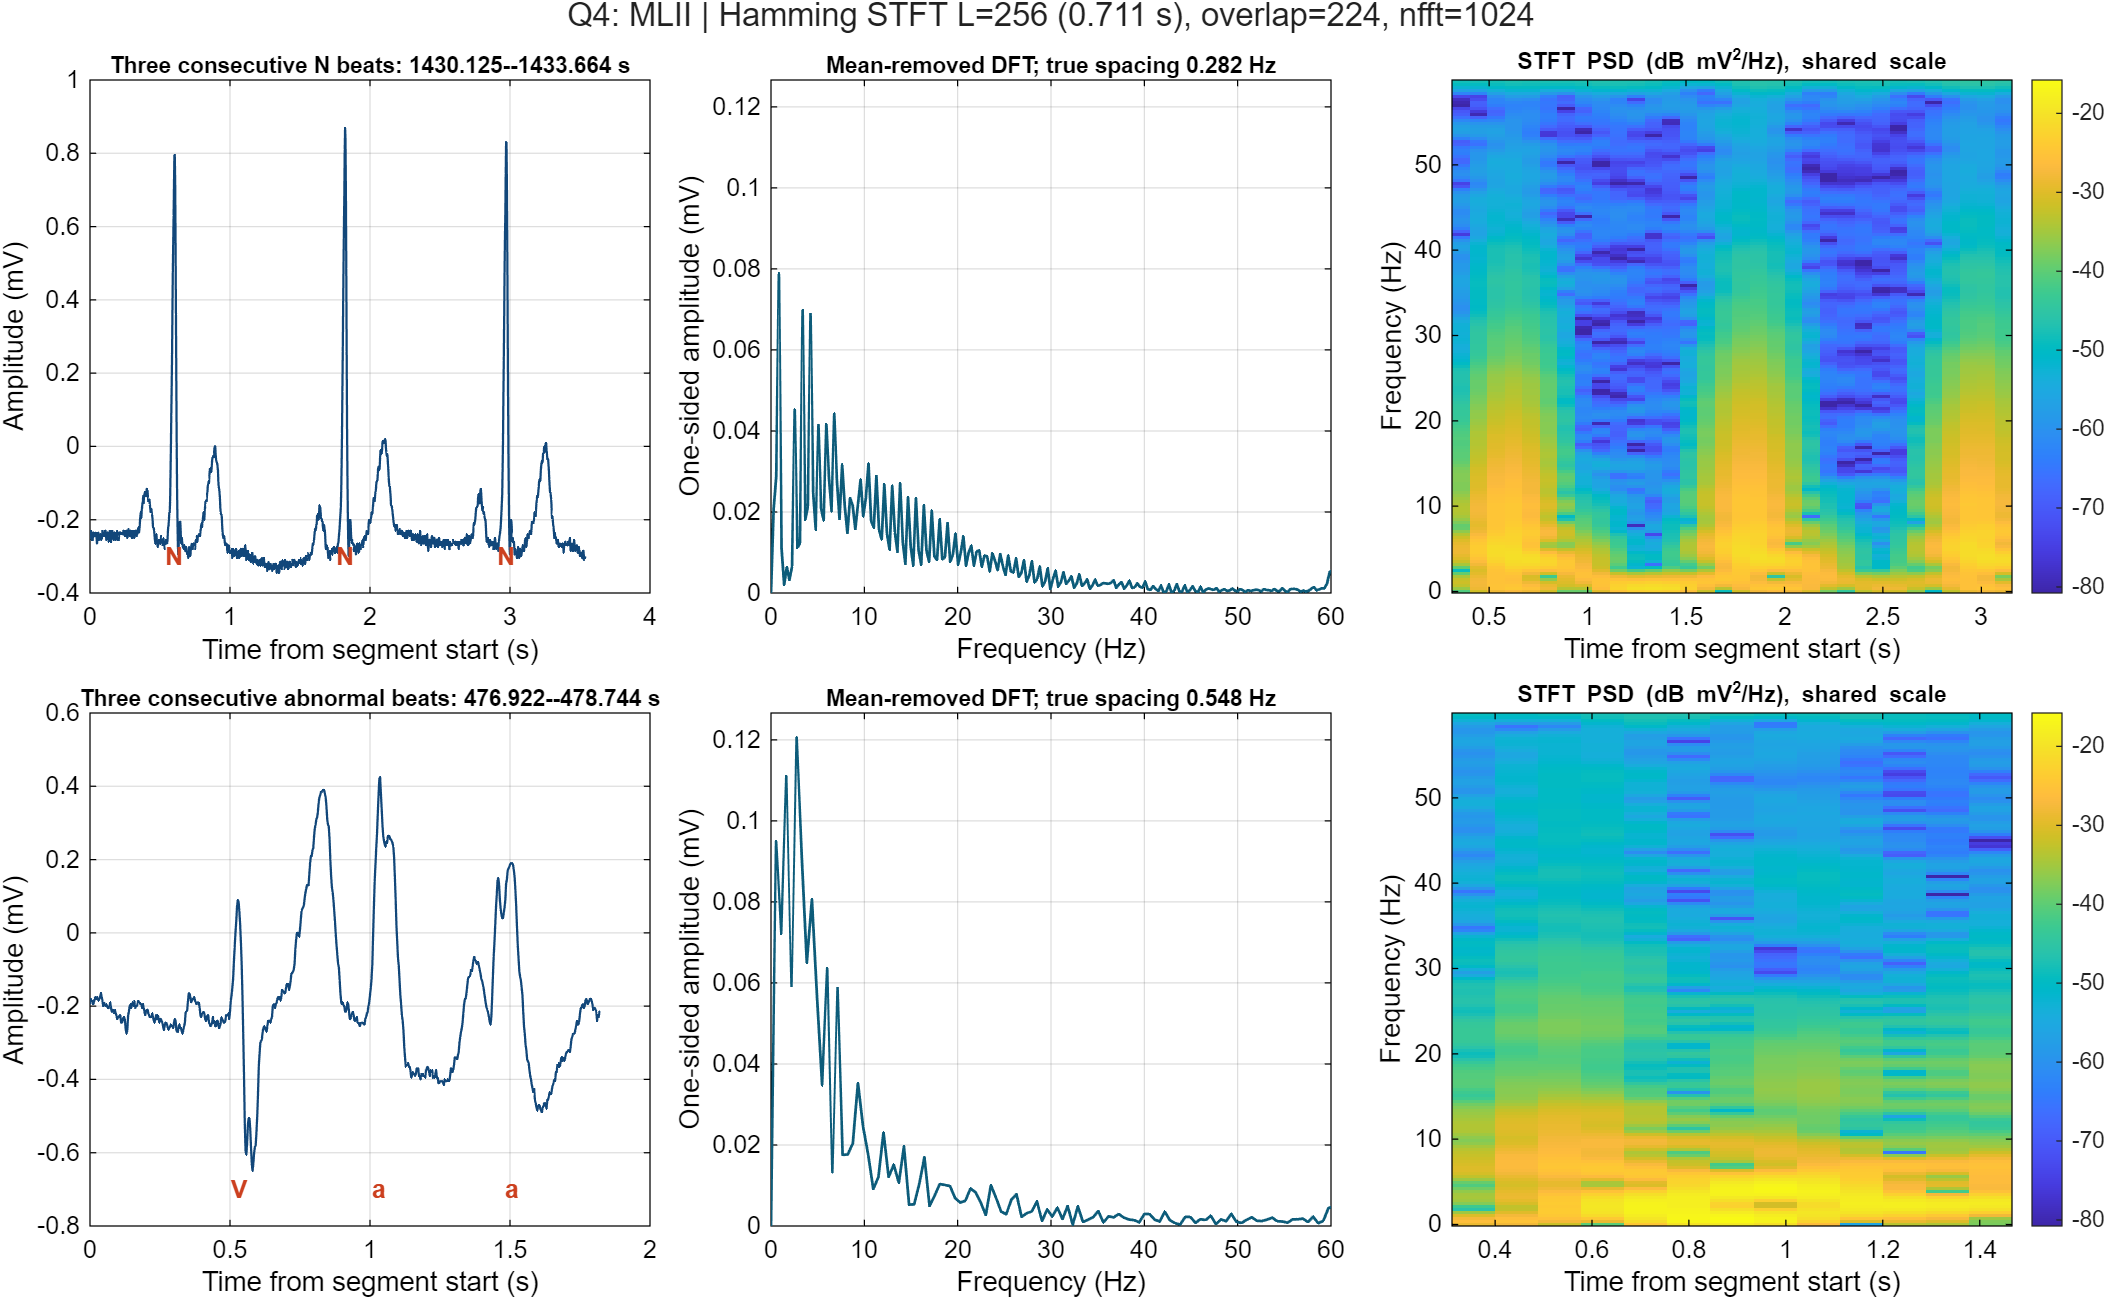
\includegraphics[width=\textwidth]{fig18_three_beats_mlii.png}
\caption{Time and spectral comparison of the two three-beat segments in the first lead.}
\label{fig:three1}
\end{figure}

In the first lead, the frequency covering 95\% of the Welch power is about 19.86~Hz for the normal segment and 10.46~Hz for the abnormal segment. Despite the shorter interval between the beats in the second segment, the power distribution of its waveform lies at lower frequencies. The rate of the beats is therefore not the same concept as the frequency of the QRS components, and it cannot be concluded that every abnormality necessarily has a higher-frequency spectrum.

\begin{figure}[H]
\centering
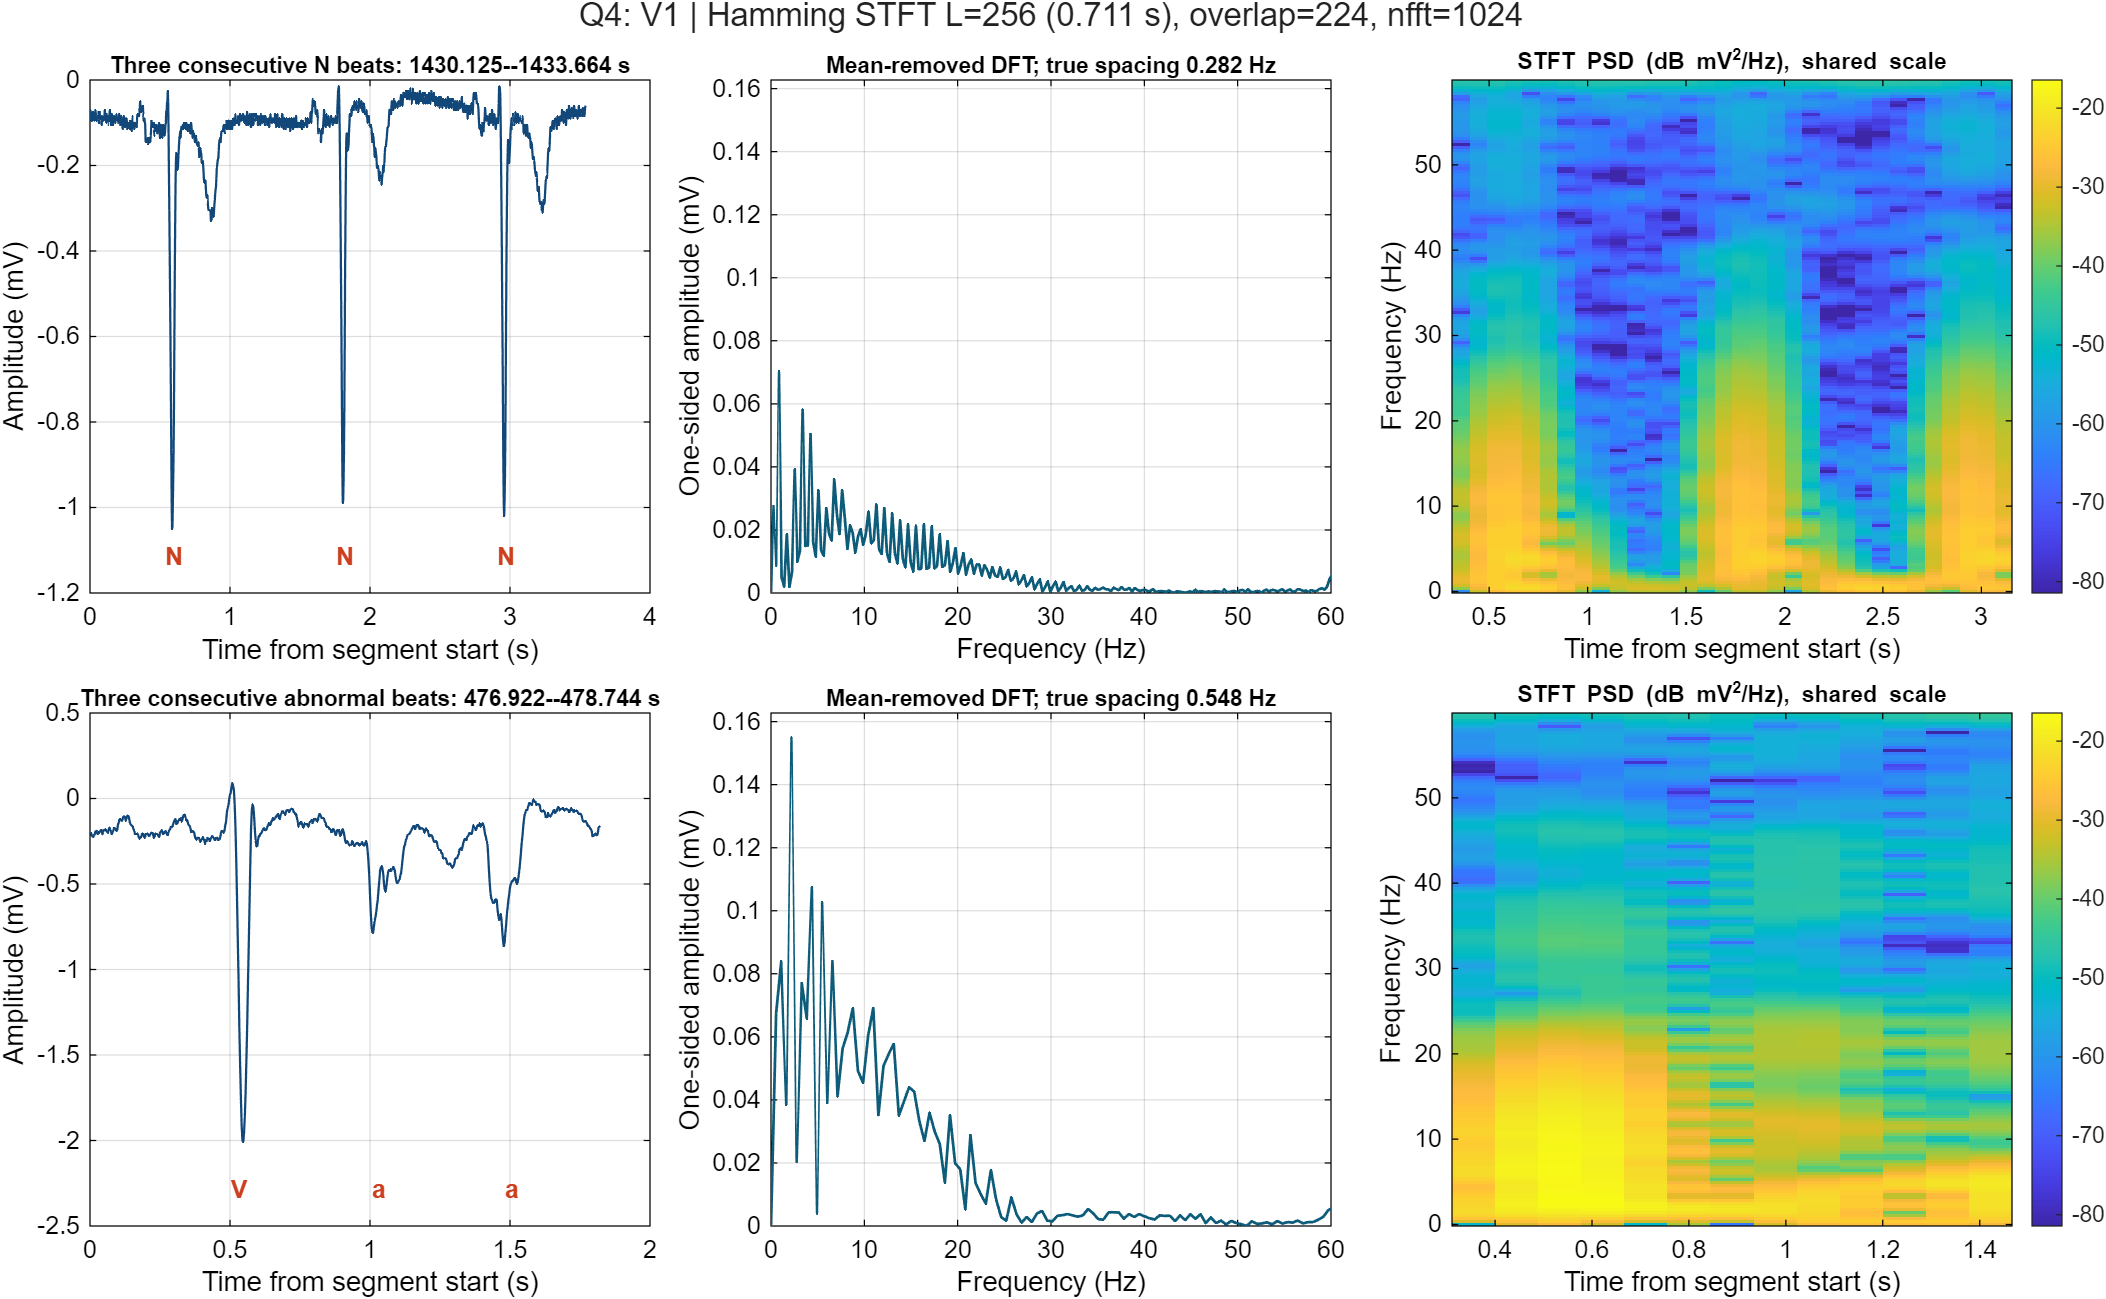
\includegraphics[width=\textwidth]{fig19_three_beats_v1.png}
\caption{Time and spectral comparison of the same two segments in the second lead.}
\label{fig:three2}
\end{figure}

In the second lead, the frequency covering 95\% of the power is about 19.60~Hz for the normal segment and 17.40~Hz for the abnormal one. The difference from the first lead results from the change in the spatial view of the cardiac activity and in the waveform shape. The spectrogram shows the temporal difference between the initial V beat and the two subsequent a beats; the overall transform sums these differences up over the whole segment. The shortness of the segments increases the fluctuation of the spectral estimate, and these results are limited to the same two segments.

\subsection{Core Implementation (ECG)}

\begin{lstlisting}[language=Matlab]
t = (0:size(Sig,1)-1)'/sfreq;     % Do not use mismatched TIME
beatCodes = [1:13 25 30 34 35 38 41];
isQRS = ismember(ANNOTD,beatCodes);
beatTimes = ATRTIMED(isQRS);
RR = diff(beatTimes);             % Excludes rhythm/quality/blocked P
\end{lstlisting}

This separation prevents the counting of non-beat events and the generation of a false heart rate. The table of the times of all events and the table of the times of the real beats are stored as two separate files in the \texttt{results} folder, and the complete code is in \texttt{code/lab1\_ecg.m}.
